\documentclass{gapd}

\Type{自助出版}
\Title{平行可變的間隙限制最長共同子序列 \\ Parallel Variable Gapped Longest Common Sequence}

\Author{Shiang-Yun Yang}{National Taiwan University}

\Author{Morris Yang}{National Taiwan University}

\Author{Stephanie Dola}{National Taiwan University}

\Abstract{可變的間隙限制最長同子序列應用於基因、分子生物學中。在之前所有的研究,已經提出在 $O(nm \alpha(n))$ 時間內的算法,其中使用了高效的遞增後綴最大值詢問,可以在 $O(\alpha(n))$ 解決每一詢問。原先的序列算法無法以直觀的方式平行,我們修改了原本算法的資料結構,並且提出平行版本的遞增任意區間最大值詢問,平行的運行時間為 $O(nm / p + n \log n)$。在單一處理器上,理論的時間複雜度可以達到 $O(nm)$ 勝過於先前的研究。

\begin{quote}\itshape
  「專注於足下,才能走得更遠」 -- 真正的名言是「千里之行,始於足下」,然而某一次意外地把足下放在前面,就在人生上留下了更多的污點。
\end{quote}

}

\Issue{1}{1}{2017}
%\Pages{35}{37}

\begin{document}
\maketitle

\section{介紹} %Introduction
\label{sec:Introduction}

最長同子序列 (\emph{longest common subsequence}) (LCS)廣泛地使用在各個應用上。在多核心平台下,大多數的研究專注於如何高效率地在波前平行,而 Jiaoyun Yang ~\cite{jiaoyun} 提出的論文中改變一般的 LCS 遞迴定義以得到更好快取使用率。這裡,我們使用相關的理論來改善在 Iliopoulos ~\cite{iliopoulos} 提及的約束條件下的 LCS,如 \emph{fixed gap LCS } (FGLCS)要求任兩個挑選的距離在相對應的另一個字串中相等,同時距離最大為 $k+1$,可在時間複雜度在 $O(nm)$ 內解決,其中 $n$, $m$ 分別為兩個輸入的字串長度。

在眾多的約束條件類型中,我們將在這篇論文針對 \emph{variable gap LCS} (VGLCS) 進行探討。在 VGLCS 中,對各個不同的位置提供約束限制,如目前給定兩個字串 $A = \tt{RCLPCRR}$, $B = \tt{RPPLCPLRC}$,各自的約束限制為 $G_A = [2, 3, 0, 0, 3, 2, 2]$ 和 $G_B = [2, 0, 0, 0, 3, 0, 0, 2, 3]$,其中 $G_A(i)$ 表示當挑選第 $i$ 個位置時,與前一個挑選的位置最多差 $G_A(i)+1$,挑選的方式如圖 ~\ref{fig:VGLCSex}。這個問題已在 Yung-Hsing Peng ~\cite{yunghsing} 的論文針對 VGLCS 提出 $O(nm \alpha(n))$ 的解法。

這一篇論文,我們將在第 \ref{??} 節部分將 Yung-Hsing Peng ~\cite{yunghsing} 提出的算法進行平行化。次著,在第二節 ~\ref{sec:parallelSerial},我們將藉由快取忘卻 (cache-oblivious) 技術,在實作上提供更好的效能。接著,在第三節 ~\ref{sec:parallelIntervalQuery} ,在理論分析上提供易平行且時間複雜度 $O(nm)$ 的設計。最後,我們總結實驗結果與理論實務上的差異。

\begin{figure}[!thb]
  \centering
  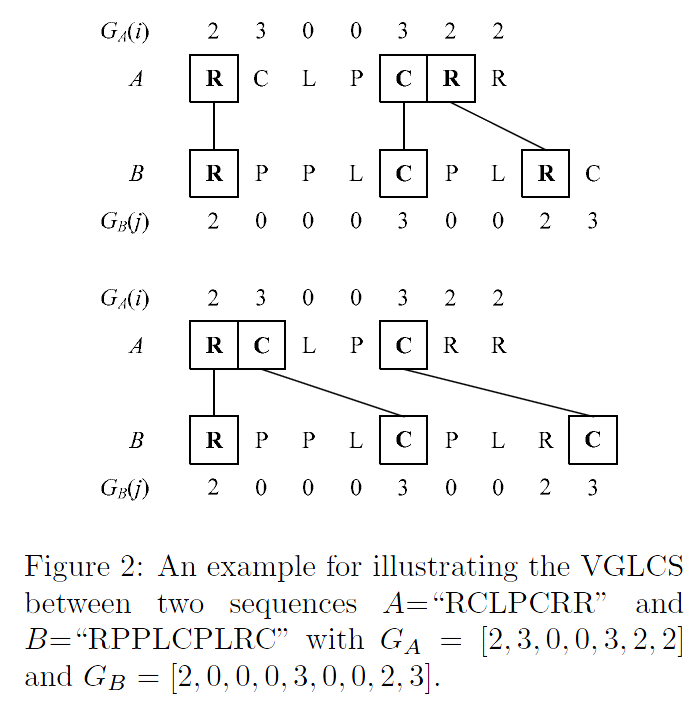
\includegraphics[height=5cm]{figure/fig-VGLCS-ex.png} % width=\linewidth,
  \caption{簡單的 VGLCS 於兩個序列 $A = \tt{RCLPCRR}$, $B = \tt{RPPLCPLRC}$,各自的約束限制為 $G_A = [2, 3, 0, 0, 3, 2, 2]$ 和 $G_B = [2, 0, 0, 0, 3, 0, 0, 2, 3]$,的其中幾個可挑選的方案}
  \label{fig:VGLCSex}
\end{figure}

\section{平行化序列算法} %
\label{sec:parallelSerial}

在 $O(nm)$ 的序列算法中 (參照算法 ~\ref{alg:serial}),我們發現算法如大多數的變型 LCS 相同,依賴左上角區塊的狀以轉移當前狀態,大量的資料依賴性不易於細粒度平行。使用波前運行平行是一種常見的解決方案,由於這種平行對於運行時的快取不友善 (cache-unfriendly),所以在 Saeed Maleki~\cite{saeed} 論文中提到如何使用 Rank Convergence 的特殊性質,拓展出更高平行度來解決動態規劃的相關問題。

\begin{algorithm*}[!thb]
  \caption{Algorithm for Finding VGLCS}
  \label{alg:serial}
  \begin{algorithmic}[1]
    \Require
      $A, B$: the input string;
      $G_A, G_B$: the array of variable gapped constraints;
    \Ensure Find the LCS with variable gapped constraints
    \State \tt{ISMQ} $Q[n]$
    \State \tt{int} $V[n][m]$
    \For{$i = 1$ to $n$}
      \State \tt{ISMQ} $RQ$
      \For{$j = 1$ to $m$}
        \If{$A[i] = B[j]$}
            \State $V[i][j] = RQ.get(j - \min(GB[j]+1, j))+1$
            \State $RQ.set(j, Q[j].get(r))$
            \State $Q[j].set(i, tmp)$
        \Else
            \State $V[i][j] = 0$
            \State $RQ.set(j, Q[j].get(r))$
        \EndIf
      \EndFor
    \EndFor
    \State Retrieve the VGLCS by tracing $V[n][m]$
  \end{algorithmic}
\end{algorithm*}

序列算法的空間複雜度為 $O(nm)$。若使用波前平行,需要同時維護橫向的所有狀態,需要多付出一倍的空間量。若加入 Rank Convergence 的想法拓展出,勢必要記錄轉移的狀態,需要耗費更多的記憶體空間,用以在最後階段合併所用。

這裡我們著手設計算法空間複雜度常數小,並且針對快取友善。從序列算法中,發現在橫向查找中使用 $O(\alpha(n))$ 操作的後綴最大值查找,這部分難以平行化。為了消除資料相依性,我們找到幾種區間詢問的替代方案。如 

\begin{itemize}
  \item Binary Indexed Tree -- $O(\log n)$: 對於任意前綴查找極值和更新元素,可以提供每次時間複雜度 $O(\log n)$,其運行常數比 Range Tree 低,但只能支持前綴查找,若要運行區間查找,則必須在數學上符合加法法則。
  \item Range Tree -- $O(\log n)$: 支持更高維度的正交區塊搜索,而我們用在區間極值查找需要 $O(\log n)$ 的時間完成所有操作。
  \item Sparse Table -- $O(n \log n)$ -- $O(1)$:
    建立表格 $T[i][j]$ 表示區間 $(i-2^j,i]$ 之間的極值。建表時間複雜度 $O(n \log n)$,對於任意區間詢問可以拆分兩個 super-block 的表格檢索,轉換過程和存取時間需要 $O(1)$。
\end{itemize}

根據 VGLCS 動態規劃時的單調性質,可以使用 Van Emde Boas Tree 作為輔助資料結構在 $O(\log \log n)$ 時間內完成操作。其中 Sparse Table 是我們認為最好的替代方案,其整合後的平行算法如下 ~\ref{alg:parallel},其時間複雜度為 $O(n^2 / p + n \log n)$,其中 $p$ 為處理器個數。

\begin{algorithm*}
  \caption{Parallel Algorithm for Finding VGLCS}
  \label{alg:parallel}
  \begin{algorithmic}[1]
    \Require
      $A, B$: the input string;
      $G_A, G_B$: the array of variable gapped constraints;
    \Ensure Find the LCS with variable gapped constraints
    \State \tt{ISMQ} $Q[n]$
    \State \tt{int} $V[n][m]$
    \For{$i = 1$ to $n$}
      \State SparseTable $sp$
      \ParFor{$j = 1$ to $m$}
        \State $sp[j] = Q[j].get(r)$
      \EndParFor
      \State sp.parallel\_build(m) -- $O(n/p \log n + \log n)$
      \ParFor{$j = 1$ to $m$}
        \If{$A[i] = B[j]$}
            \State $V[i][j] = sp.get(j - \min(GB[j]+1, j), j-1)+1$
            \State $Q[j].set(i, V[i][j])$
        \EndIf
      \EndParFor
    \EndFor
    \State Retrieve the VGLCS by tracing $V[n][m]$
  \end{algorithmic}
\end{algorithm*}

\section{平行區間查詢} %
\label{sec:parallelRMQ}

\subsection{背景}

縱使我們已能很好地平行化原本的序列算法,在理論複雜度上受限於平行下的區間極值查詢 (Range Minimum/Maximum Query, RMQ)。在這個應用中,每一階段有 $n$ 個元素和 $n$ 個區間詢問。這樣的條件下,大部分樹狀結構難以在前處理過程或者每次詢問達到最好效能,對於 $O(n)$ -- $O(1)$ 操作的離線區間詢問無法提供平行,而大多數的情況下,它們依賴笛卡爾樹 (Cartesian tree) 和塔揚離線最小共同祖先算法 (Tarjan's off-line lowest common ancestors algorithm),再接續的小節中,我們將提出在兼顧兩者的平行算法。

\subsection{快取忘卻笛卡爾樹}

在 Fischer ~\cite{fischer} 的論文中,已經優化 RMQ 和 LCA 問題,根據卡塔蘭數 $\frac{1}{s+1}\binom{2s}{s} = O(\frac{4^s}{s^{1.5}})$ 建立查找表 (lookup-table)。當我們選擇 $s = \frac{1}{4} \log n$ 時,空間複雜度 $O(s^2 \frac{4^s}{s^{1.5}}) = o(n)$ 且建表複雜度 $o(n)$。每一個區間詢問將會拆成 2 個 super-block 和 2 個 in-block 詢問 (參照圖 ~\ref{??}),共計需要 4 次的記憶體存取。在理論分析上,離線的 RMQ 問題已經可以在 $\theta(n)$ -- $\theta(1)$ 時間內解決任何詢問。

當 $n$ 越大時,這 4 次的記憶體存取會遭遇到嚴重的快取未中 (cache miss),在 Demaine ~\cite{demaine} 的論文中,發展出快取忘卻 (cache oblivious) 形式的查找方案,降低在離線版本中的 in-block 詢問產生的快取未中。

在上述的技術中,我們可以藉由 Fischer 提出的方案平行化 RMQ 至 $O(n / p + \log n)$ -- $O(1)$,使用 Demaine 提供的技巧壓縮空間使用量,降低快取未中以提升運行效能。這裡我們挑選固定長度的壓縮方案,選擇每 16 個整數壓縮成一棵笛卡爾樹。在第 $i$ 次插入時,左旋的次數 $l_i$,每次操作皆符合 

$$\sum_{i=1}^{n} l_i < i$$

因此所有 $l_i < 16$,每個 $l_i$ 使用 4-bit 表示之,最後用 64-bit 表示整個笛卡爾樹。為了現在常見的 64-byte 快取列 (cache line) 和 64-bit 暫存器 (register) 考量,我們選用合適的大小進行測試,不僅壓縮空間使用量,同時也減少快取未中的問題。請參考 ~\ref{alg:cacheObliviousTransfer}。

\begin{algorithm*}
  \caption{Transfer Cartesian Tree to 64-bits with 8 integers}
  \label{alg:cacheObliviousTransfer}
  \begin{algorithmic}[1]
    \Require
      $A[1 \cdots 16]$: 16 integers store in array
    \Ensure 
      $\textit{tmask}$: compress Cartesian tree into 64-bits integer
      \State $\tt{LOGS} = 4$
      \State $\tt{POWS} = 2^{\tt{LOGS}}$
      \State int $D[POWS+1]$, $Dp = 0$;
      \State uint64\_t $tmask$ = $0$
      \State $D[0]$ = SHRT\_MAX
      \For{$i = 1$ to $\tt{POWS}$} 
        \State $v = A[i]$;
        \State $cnt = 0$;
        \While{$D[Dp] < v$}
          \State $Dp = Dp-1$
          \State $cnt = cnt + 1$
        \EndWhile
        \State $Dp = Dp+1$
        \State $D[Dp] = v$
        \State $tmask = tmask | ((cnt)<<((i-1)<<2))$
      \EndFor
      \State return $tmask$
  \end{algorithmic}
\end{algorithm*}

\begin{algorithm*}
  \caption{Range Minimum Query in 64-bits Cartesian Tree}
  \label{alg:cacheObliviousQuery}
  \begin{algorithmic}[1]
    \Require
      $\textit{tmask}$: 64-bits Cartesian tree;
      $[l, r]$: query interval between $l$ and $r$
    \Ensure 
      $\textit{minIdx}$: the index of the minimum value in interval
    \State int $\textit{minIdx}$ = $l$, $x$ = $0$;
    \For{$l = l+1$ to $r$}
      \State $x$ = $x+1 - ((tmask>>(l<<2))\&15)$
      \If{$x \le 0$}
        \State $\textit{minIdx}$ = $l$
        \State $x$ = $0$
      \EndIf
    \EndFor
    \State return $\textit{minIdx}$
  \end{algorithmic}
\end{algorithm*}

然而在我們的應用中,僅能在內層迴圈使用這個技巧,時間複雜度從 $O(n^2 / p + n \log n)$ 降到 $O(n^2 \alpha(n) / p + n \alpha(n))$,這已經達到近乎序列算法平行度的理想。再接續的章節中,我們將更進一步地將 $o(\alpha(n))$ 降到 $o(1)$。

\subsection{動態笛卡爾樹標記與區間詢問}

在 VGLCS 問題中,主要分成縱向和橫向兩階段,縱向處理每一列的區間極值查找,橫向處理每一行的區間極值查找,兩者合併構成區域極值查找。在縱向方面為數個獨立的數據結構,因此很容易平行;相反地,在橫向方面,需要共同協作一個數據結構。綜觀這兩者的差異,縱向需要動態的後綴插入和區間查詢,而橫向可以離線完成區間查找。在上一節中,我們提出在橫向處理的實作,若限制上述的實作方案在單一處理器上,時間複雜度的瓶頸將受限於縱向的更新與查找。最後,我們的成果如表 ~\ref{tab:cmpComplexity} 所示。

\begin{table}
  \tiny
  \centering
  \begin{tabular}{ccc}
    \toprule
     & serial & parallel \\
    \midrule
    horizontal & \begin{tabular}{@{}c@{}}
              $\left \langle n \alpha(n) \right \rangle$ \cite{yunghsing} \\ 
              amortized $\left \langle n \right \rangle$\end{tabular}
              & \begin{tabular}{@{}c@{}}
                $\left \langle n \alpha(n)/p + \alpha(n) \right \rangle$ \cite{yunghsing} \\
                amortized $\left \langle n /p + o(1) \right \rangle$
                \end{tabular} \\
    vertical & \begin{tabular}{@{}c@{}}
                $\left \langle n \alpha(n) \right \rangle$ \\
                amortized $\left \langle n \right \rangle$
                \end{tabular}
            & \begin{tabular}{@{}c@{}}
                impossible \\
                amortized $\left \langle n /p + o(1) \right \rangle$
              \end{tabular}
              \\
    total & \begin{tabular}{@{}c@{}}
              $\left \langle n^2 \alpha(n) \right \rangle$ \cite{yunghsing} \\ 
              amortized $\left \langle n^2 \right \rangle$\end{tabular}
          & \begin{tabular}{@{}c@{}}
              impossible \\ 
              amortized $\left \langle n^2 /p + n \log n \right \rangle$\end{tabular} \\
    \bottomrule
  \end{tabular}
  \caption{我們的研究成果如粗體字所述,均攤部分將在 $s=16$ 的笛卡爾樹上,整理影響的常數很小,不易遇到負載平衡上的問題。}
  \label{tab:cmpComplexity}
\end{table}

\subsubsection{平行建立查找表}

為解決縱向平行處理,我們從 Fischer \cite{fischer} 和 Masud \cite{masud} 的研究中,分別得到關於笛卡爾的編碼與快取改善的技術。然而,這些技術都著手於離線操作,意即必須先知道 $n$ 個元素值為何,在 $O(n)$ 時間內編碼一棵樹,接著,再利用前處理的查找表完成極值查找;從這些觀點出發,我們將提出動態的編碼方式。

我們採用字典順序的方式編碼一棵樹,優先增長左子樹,當相同左子樹時,增長右子樹的方式進行編號,其編碼方式可參考圖 ~\ref{fig:lablingBST}。

\begin{figure}[!thb]
  \tikzset{
  treeInode/.style = {align=center, inner sep=1pt, text centered,
    font=\sffamily},
  arn_n/.style = {treeInode, rectangle, rounded corners=1mm, black, draw=black, fill=black, text=white, font=\sffamily\bfseries, minimum width=1em, minimum height=1em}
    % arbre rouge noir, noeud noir
}
\usetikzlibrary{patterns}

\begin{tikzpicture}[-,>=stealth',level/.style={sibling distance = 0.5cm/#1,
  level distance = 0.6cm}]
\node[arn_n]{0}
; 
\node[below=0.2cm, align=flush center,text width=1cm]{$0$};
\end{tikzpicture}
  \begin{tikzpicture}[-,>=stealth',level/.style={sibling distance = 0.6cm,
  level distance = 0.4cm}]
\node[arn_n]{\tiny $1$}
  child{
    node[arn_n]{\tiny $0$}
  }
  child[missing]{
  }
; 
\node[below=1cm, align=flush center,text width=1cm]{\small $0$};
\end{tikzpicture}
\begin{tikzpicture}[-,>=stealth',level/.style={sibling distance = 0.6cm,
  level distance = 0.4cm}]
\node[arn_n]{\tiny $0$}
	child[missing]{
	}
	child{
		node[arn_n]{\tiny $1$}
	}
; 
\node[below=1cm, align=flush center,text width=1cm]{\small $1$};
\end{tikzpicture}
  \begin{tikzpicture}[-,>=stealth',level/.style={sibling distance = 0.5cm/#1,
  level distance = 0.6cm}] 
\node[arn_n]{2}
  child{
    node[arn_n]{1}
    child{
      node[arn_n]{0}
    }
    child[missing]{
    }
  }
  child[missing]{
  }
; 
\node[below=1.5cm, align=flush center,text width=0.5cm]{$0$};
\end{tikzpicture}
\begin{tikzpicture}[-,>=stealth',level/.style={sibling distance = 0.5cm/#1,
  level distance = 0.6cm}] 
\node[arn_n]{2}
  child{
    node[arn_n]{0}
    child[missing]{
    }
    child{
      node[arn_n]{1}
    }
  }
  child[missing]{
  }
; 
\node[below=1.5cm, align=flush center,text width=0.5cm]{$1$};
\end{tikzpicture}
\begin{tikzpicture}[-,>=stealth',level/.style={sibling distance = 0.5cm/#1,
  level distance = 0.6cm}] 
\node[arn_n]{1}
  child{
    node[arn_n]{0}
  }
  child{
    node[arn_n]{2}
  }
; 
\node[below=1.5cm, align=flush center,text width=0.5cm]{$2$};
\end{tikzpicture}
\begin{tikzpicture}[-,>=stealth',level/.style={sibling distance = 0.5cm/#1,
  level distance = 0.6cm}] 
\node[arn_n]{0}
  child[missing]{
  }
  child{
    node[arn_n]{2}
    child{
      node[arn_n]{1}
    }
    child[missing]{
    }
  }
; 
\node[below=1.5cm, align=flush center,text width=1cm]{$3$};
\end{tikzpicture}
\begin{tikzpicture}[-,>=stealth',level/.style={sibling distance = 0.5cm/#1,
  level distance = 0.6cm}] 
\node[arn_n]{0}
  child[missing]{
  }
  child{
    node[arn_n]{1}
    child[missing]{
    }
    child{
      node[arn_n]{2}
    }
  }
; 
\node[below=1.5cm, align=flush center,text width=0.5cm]{$4$};
\end{tikzpicture}
  \caption{Labeling Binary Search Tree}
  \label{fig:lablingBST}
\end{figure}

對於 $n$ 個節點的二元搜尋樹,有卡坦蘭數 $C_n$ 個不同的型。對於 $n$ 個節點的樹,其權重從 $0$ 開始至 $n-1$、樹編號為 $\mathit{tid}$,定義 $\mathit{LCA}(n, \mathit{tid}, p, q)$ 為其樹上兩點 $p$ 和 $q$ 的最小共同祖先。從遞迴公式中,額外定義四個變數 $\langle\mathit{lsz},\mathit{lid},\mathit{rsz},\mathit{rid}\rangle$ 為左右子樹的大小和其編號,這四個變數在 $O(n)$ 時間內完成。最後,我們得到遞迴公式如式 ~\ref{fig:formulaLCA}。 

\begin{figure*}[!thb]
\begin{equation*}
  \begin{split}
    &\mathit{LCA}(n, \mathit{tid}, p, q) \\
      &= \left\{\begin{matrix*}[l]
        \mathit{LCA}(\mathit{lsz}, \mathit{lid}, p, q) &&, p \le q < \mathit{lsz}\\ 
        \mathit{LCA}(\mathit{rsz}, \mathit{rid}, p-\mathit{lsz}-1, q-\mathit{lsz}-1)+\mathit{lsz}+1 &&, 
            \mathit{lsz} \le p \le q < n \\ 
        \mathit{lsz} && , 0 \le p \le \mathit{lsz}, \mathit{lsz} \le q \le i\\ 
        -1 && ,\mathit{otherwise}
      \end{matrix*}\right.
  \end{split}
\end{equation*}
\caption{Recursion Formula for labeling BST}
\label{fig:formulaLCA}
\end{figure*}

這張表使用 $\theta\left(\frac{n^2}{n+1} \binom{2n}{n}\right)$ 空間,搭配 RMQ 問題,使得大部分的應用讓 $n \le 8$,因此空間消耗上可以允許的。建立這張表的平行算法如 ~\ref{alg:parallelLCA},其平行複雜度如下:

$$\theta\left(s^3 \; \frac{1}{s+1} \binom{2s}{s} \bigg/ p + s^2 \right)$$

\begin{algorithm*}
  \caption{Parallel Algorithm for building LCA}
  \label{alg:parallelLCA}
  \begin{algorithmic}[1]
    \Require
      $s$: Maximum size for required the number of BST
    \For{$n = 1$ to $s$}
      \ParFor{$\mathit{tid} = 0$ to $C_n - 1$}
        \ParFor{$p = 0$ to $n-1$}
          \State compute $\langle\mathit{lsz},\mathit{lid},\mathit{rsz},\mathit{rid}\rangle$ in $O(n)$
          \For{$q = p$ to $n-1$}
            \State LCA[$n$][$\mathit{tid}$][$p$][$q$] = $\cdots$ ~\ref{fig:formulaLCA}
          \EndFor
        \EndParFor
      \EndParFor
    \EndFor
  \end{algorithmic}
\end{algorithm*}

在這應用下,詢問次數與元素個數相當,故無法像 Masud \cite{masud} 的研究來減少快取未中的問題,只能依賴數據本身的分佈和編碼之間的關聯來減少快取未中的情況。

\subsubsection{動態編碼笛卡爾樹}

在我們的應用中維護後綴最大值,其操作需要以下兩者:

\begin{itemize}
  \item \texttt{Append V} : 插入元素 $V$ 至陣列 $A$ 的尾端
  \item \texttt{Query L R} : 詢問 $A[L .. R]$ 中的最大值
\end{itemize}

已知解法有二,其一使用並查集在 $O(\alpha(n))$ 解決單一操作,其二使用樸素的稀疏表在 $O(\log n)$完成插入操作、$O(1)$ 完成詢問操作。而 Fischer \cite{fischer} 提出的 $\theta(n)$ -- $\theta(1)$ 無法應用在此,其原因在於插入元素時,無法動態決定 in-block 的最大值,必須等到整個 in-block 塞滿至預設值才可解決。接著,我們將提供動態的編碼方式,使得每一操作皆均攤 $\theta(1)$ 完成。

我們在上一節提出對於任意編號 $\mathit{tid}$ 可以在 $O(n)$ 時間內得到 $\langle\mathit{lsz},\mathit{lid},\mathit{rsz},\mathit{rid}\rangle$;相反地,可以在 $\theta(1)$ 時間內逆推得到 $\mathit{tid}$,參考算法 ~\ref{alg:FunctionTid}。我們可以透過預處理,事先將所有前綴和保存下來,在算法 ~\ref{alg:FunctionTid} 的迴圈可視為一次內存存取。

\begin{algorithm}
  \caption{Get $tid$ from $\langle\mathit{lsz},\mathit{lid},\mathit{rsz},\mathit{rid}\rangle$ in $\theta(1)$ time}
  \label{alg:FunctionTid}
  \begin{algorithmic}[1]
    \Require
      $\langle\mathit{lsz},\mathit{lid},\mathit{rsz},\mathit{rid}\rangle$: size and label in left/right subtree
    \Ensure
      $\mathit{tid}$: this label
    \If{$\mathit{rsz} = 0$}
      \State return $\mathit{lid}$
    \EndIf
    \State $n = \mathit{lsz}+\mathit{rsz}+1$
    \State $\mathit{base} = 0$
    \For{$i=0$ to $\mathit{lsz}-1$}
      \State $\mathit{base}$ += $C_i$ * $C_{n-i-1}$
    \EndFor
    \State $\mathit{offset}$ = $\mathit{lid}$ * $C_{\mathit{rsz}}$ + $\mathit{rid}$
    \State return $\mathit{base}$ + $\mathit{offset}$
  \end{algorithmic}
\end{algorithm}

根據先前的字典順序編碼,只需要維護笛卡爾樹的右鏈,其實作上與堆疊結構相同。基於 row-major 的順序和遞迴定義 ~\ref{alg:FunctionTid},修改之前論文對於的離線編碼,其對應方案如下 ~\ref{alg:typeOfCartesianOffline}:

\begin{algorithm*}
  \caption{Offline Type of Cartesian Tree}
  \label{alg:typeOfCartesianOffline}
  \begin{algorithmic}[1]
    \Require
      $A[1 \cdots s]$: storage array;
      $s$: the number of elements;
    \Ensure
      $\mathit{tid}$: this label
    \State $\langle\mathit{lsz},\mathit{lid},\mathit{value}\rangle$ $D$[$s+1$]
    \State Dp = 0
    \State $D$[0] = $\langle0,0,\infty\rangle$
    \For{$i = 1$ to $s$}
      \State v = $A$[i], lsz = 0, lid = 0
      \While{$D$[Dp].value < v}
        \State lid = tid($D$[Dp].lsz, $D$[Dp].lid, lsz, lid)
        \State lsz += $D$[Dp].lsz + 1
        \State Dp = Dp - 1
      \EndWhile
      \State Dp = Dp + 1
      \State $D$[Dp] = $\langle\mathit{lsz},\mathit{lid},\mathit{v}\rangle$
    \EndFor
    \State lsz = 0, lid = 0
    \While{Dp > 0} // pop all
      \State lid = tid($D$[Dp].lsz, $D$[Dp].lid, lsz, lid)
      \State lsz += $D$[Dp].lsz + 1
      \State Dp = Dp - 1
    \EndWhile
    return lid
  \end{algorithmic}
\end{algorithm*}

許多研究致力於如何將編碼過程的運算量最小化,如改變遞迴定義公式,便可用數個暫存器狀態轉移取代內存存取 ... 等,這些方法皆使用離線編碼,其攤銷複雜度會到 $\theta(s)$,故不適用於後綴最大值查找。

為了支持動態編碼,我們提出攤銷 $\theta(1)$ 的算法。首先,我們定義轉移狀態由 5 個變數決定,當前插入第 $i$ 個元素,最終填充 $s$ 個元素,當前的樹編號 $\mathit{tid}$,以及笛卡爾樹的右鏈狀態指針 $Dp$ 與其堆疊 $D$,其結構如下:

\begin{lstlisting}
struct State {
  int i, s, tid, Dp
  <lsz,lid,value> D[s+1]
}
State 
  init(i = 0, s = n, tid = C[n]-1, 
          D[0].value = INF, Dp = 0)
\end{lstlisting}

為了解決詢問操作,我們必須搭配 Fischer \cite{fischer} 的研究,取 $s = \frac{1}{4} \log n$ 使得整體落在 $\theta(n)$,提出的在線編碼算法 ~\ref{alg:typeOfCartesianOnline} 只存取 $s$ 個節點的 LCA 表,而非隨著插入元素的增加,則存取 $[1, s]$ 的 LCA 表,故一開始建立虛設點 $s$ 個在右鏈上,其樹編號 $\mathit{tid} = C_n - 1$。隨著插入元素的增加,尚未加入的元素都預設嚴格遞減,加上根據編碼順序,我們藉由差值來維護在線編碼 (參考圖 ~\ref{??})。最後,我們不改變原本的建立笛卡爾樹算法,又能在過程中擭得樹的編號,忽略建表所需時間,每一次的 in-block 詢問將查找表,得到任一操作攤銷複雜度 $\theta(1)$。

\begin{algorithm*}
  \caption{Online Type of Cartesian Tree}
  \label{alg:typeOfCartesianOnline}
  \begin{algorithmic}[1]
  \Require
      $\mathit{state}$: state of Cartesian Tree;
      $v$: the value which append to array
  \Ensure
      $\mathit{tid}$: this label
  \State Dp = state.Dp, lsz = lid = 0
  \State bsz = state.s - state.i + 1
  \State bid = C[bsz] - 1 
  \While{state.D[Dp].value < v}
    \State lid = tid(state.D[Dp].lsz, state.D[Dp].lid, lsz, lid)
    \State bid = tid(state.D[Dp].lsz, state.D[Dp].lid, bsz, bid)
    \State lsz = lsz + state.D[Dp].lsz+1
    \State bsz = bsz + state.D[Dp].lsz+1
    \State Dp = Dp - 1
  \EndWhile
  \State Dp = Dp + 1
  \State state.D[Dp] = <lsz,lid,v>, state.Dp = Dp
  \State state.tid = state.tid + bid - tid(lsz, lid, state.s-state.i, C[state.s-state.i]-1)
  \State state.i = state.i + 1
  \State return state.tid
  \end{algorithmic}
\end{algorithm*}

\section{實作細節}
\label{sec:Implementation}

\subsection{平行并查集操作策略}

運行 VGLCS 時,將耗費 $\theta(n^2)$ 的內存空間。使用遞增後綴最大值 (ISMQ) 時,採用並查集實作將會遭遇到很多不平衡的工作負載,其原因在於合併的策略,常見的有路徑壓縮和啟發式合併兩種策略,這間接影響到不同次數的分枝判斷。實務上須考慮到快取未中,故兩種策略只能擇其一,兩者皆用將引發更多的快取未中而導致效能下滑。

數個執行緒分配到獨立的并查集,操作時偏向延遲標記操作,儘早合併的策略易造成快取未中。由於動態規劃的傾向中,插入值的趨勢有兩種情況,其一為連續不合定義的零元素插入,其二為遞增元素的插入,在這兩者穿插的趨勢中,我們發現延遲操作將會帶來較能改善快取未中問題。

\subsection{平行區間查找策略}

一般運行區間查找時,依賴內建函數 \texttt{\_\_builtin\_clz} 在 $O(1)$ 時間完成,然而在 VGLCS 中,區間查找的對數結果都是可以被預測的,預先將每一組詢問的區段對數結果儲存在陣列中,便可降低運行常數。

由於已知所有詢問區間,建立稀疏表時,可藉由動態規劃在 $O(n \log n)$ 排除掉不可能的計算,降低過程中的計算量。由於 VGLCS 在平行操作需要 $O(n \log n)$,故使用動態規劃不影響我們的最終結果。

由 Fischer \cite{fischer} 提出的策略中,雖 in-block 詢問可藉由笛卡爾樹的編號 $O(1)$ 查找,查找表易引發快取未中。從機率分佈的角度來看,因 $s = \frac{1}{4} \log n$ 過小,區間詢問完全落於 block 的機率低,故額外維護區段前綴和後綴最大值 (prefix/suffix maximum value in block) 取代笛卡爾樹的建立。

\section{實驗結果}
\label{sec:Experiment}

我們運行在 Intel Xeon E5-2620 2.40 GHz 主機上,其擁有 L1 cache 384 KiB、L2 cache 1536 KiB 和 L3 cache 15 MiB。

\subsection{空間壓縮 VGLCS}

我們運行優化策略中的空間壓縮版本,而非理論分析的 $\theta(1)$ 操作,單次詢問落在 $O(s)$ 中,在實作上由於可以完全壓在暫存器上操作,效能表現較佳。

\begin{figure}[!thb]
  \centering
  \documentclass[border=2pt]{standalone}
\usepackage{tikz}
\usetikzlibrary{calc} \usetikzlibrary{positioning} \usetikzlibrary{shapes,arrows} \usetikzlibrary{plotmarks}
\usepackage{pgfplots}

\begin{document}
	\begin{tikzpicture}
		\begin{axis}[
				xlabel={Length $n$},
				ylabel={Time (second)},
				xmin=0, xmax=10000,
				ymin=0, ymax=4.5,
				scaled ticks = false,
				tick label style={/pgf/number format/fixed},
				xtick={0, 1000, 2000, 3000, 4000, 5000, 6000, 7000, 8000, 9000, 10000},
				ytick={0, 0.5, 1, 1.5, 2, 2.5, 3, 3.5, 4, 4.5},
				legend pos=north east,
				legend cell align=left,
				ymajorgrids=true,
				grid style=dashed,
				line width=1pt,
				mark size=3pt,
				height=10cm,width=15cm,
			]
			\addplot [mark=*] file{./data/serial-n.dat};
			\addplot [mark=square*, mark options={fill=white}] file{./data/parallel-n.dat};
			\legend{serial, parallel}
		\end{axis}
	\end{tikzpicture}
\end{document}

  \caption{Serial and Parallel Algorithm run on E5-2620}
  \label{fig:fig-parallel}
\end{figure}

從圖 ~\ref{fig:fig-parallel-scala} 看出,平行 VGLCS 的縮放性不佳,從 profiler 中得到快取未中的問題需要解決。

\begin{figure}[!thb]
  \centering
  \documentclass[border=2pt]{standalone}
\usepackage{tikz}
\usetikzlibrary{calc} \usetikzlibrary{positioning} \usetikzlibrary{shapes,arrows} \usetikzlibrary{plotmarks}
\usepackage{pgfplots}

\begin{document}
	\begin{tikzpicture}
		\begin{axis}[
				xlabel={Processor $p$},
				ylabel={Time (second)},
				xmin=1, xmax=16,
				ymin=0, ymax=1.2,
				scaled ticks = false,
				tick label style={/pgf/number format/fixed},
				xtick={1, 2, 4, 8, 16},
				ytick={0, 0.2, 0.4, 0.6, 0.8, 1, 1.2},
				legend pos=north east,
				legend cell align=left,
				ymajorgrids=true,
				grid style=dashed,
				line width=1pt,
				mark size=3pt,
				height=10cm,width=15cm,
			]
			\addplot [mark=square*, mark options={fill=white}] file{./data/parallel-p.dat};
			\legend{parallel $n=5000$}
		\end{axis}
	\end{tikzpicture}
\end{document}

  \caption{Scalability for our Parallel Algorithm}
  \label{fig:fig-parallel-scala}
\end{figure}

\subsection{理論常數 VGLCS}

尚未完成

\subsection{平行區間查找}

每一次有 $n$ 個元素和 $n$ 組詢問,針對這種特殊性質的問題,我們運行樸素的 \texttt{CORMQ} (cache-oblivious RMQ) 得到效能改善,搭配可預測的分析降低運算量 (參照 \texttt{CORMQ-opt}),得到更好的改善。在 \texttt{CORMQ-opt} 策略中,得到 $2.35 \times$ 倍的加速。實驗結果如表 ~\ref{tlb:CORMQ}

\begin{table}[!thb]
  \tiny
  \centering
  \begin{tabular}{l c c c c}
    \firsthline
      & \multicolumn{4}{c}{$N$} \\
      \cline{2-5}
        & \multicolumn{2}{c}{$30000$} & $50000$ & $100000$ \\
      $L$ & $2^{10}$ & $2^{15}$ & $2^{15}$ & $2^{15}$ \\
      \hline
      parallel-\tt{RMQ}     & $903$ & $1516$ & $1874$ & $4116$ \\
      parallel-\tt{CORMQ}   & $995$ & $1475$ & $1689$ & $2594$ \\
      parallel-\tt{CORMQ-opt} & $843$ & $1373$ & $1136$ & $1745$ \\
      \hline
      Speedup & $1.07\times$ & $1.10\times$ & $1.64\times$ & $2.35\times$\\
    \lasthline
  \end{tabular}
  \caption{Total running time (ms) for finding RMQ of different sizes $N$ and maximum interval sizes $L$.}
  \label{tlb:CORMQ}
\end{table}

\section{結論}
\label{sec:Conclusion}

我們修改 VGLCS 的序列算法,將其平行化於 $\theta(n \log n)$ 時間內,並以稀疏表實作 ISMQ 問題。提出的稀疏表能解決比 VGLCS 更困難的 Variable Interval Gapped LCS,致使 VIGLCS 可在時間複雜度 $\theta(nm)$ 被解決。

在實務上,我們提供以動態規劃減少計算量,以及使用空間壓縮降低快取未中的策略,最終平行 RMQ 獲取 $2.35 \times$ 倍的加速;在理論上,提出 $\theta(n)$ -- $\theta(1)$ 的實作,並且能提供附加操作的編碼策略。

\section*{致謝}

特別感謝某某

\begin{thebibliography}{4}

\bibitem{jiaoyun} Jiaoyun Yang, Yun Xu, Yi Shang, `An Efficient Parallel Algorithm for Longest Common Subsequence Problem on GPUs', Proceedings of the World Congress on Engineering, 2010, vol.~I 

\bibitem{iliopoulos} C. S. Iliopoulos and M. S. Rahman, `Algorithms for computing variants of the longest common subsequence problem', Theoretical Computer Science, 2008, vol.~395, pp. 255--267

\bibitem{yunghsing} Yung-Hsing Peng and Chang-Biau Yang, The Longest Common Subsequence Problem with Variable Gapped Constraints

\bibitem{saeed} Saeed Maleki, `Efficient Parallelization Using Rank Convergence in Dynamic Programming Algorithm', Microsoft, 2016

\bibitem{demaine} Erik D. Demaine, On Cartesian Trees and Range Minimum Queries, MIT, 2009

\bibitem{fischer} J. Fischer and V. Heun. `Theoretical and practical improvements on the RMQ-problem, with applications to LCA and LCE'. In Proceedings of the 17th symposium on Combinatorial Pattern Matching (CPM), pages 36–48, 2006.

\bibitem{masud} Masud HasanTanaeem M. MoosaM. Sohel Rahman, `Cache Oblivious Algorithms for the RMQ and the RMSQ Problems', Mathematics in Computer Science, 2010.

\end{thebibliography}

\end{document}
 